\let\negmedspace\undefined
\let\negthickspace\undefined
\documentclass[journal]{IEEEtran}
\usepackage[a5paper, margin=10mm, onecolumn]{geometry}
%\usepackage{lmodern} % Ensure lmodern is loaded for pdflatex
\usepackage{tfrupee} % Include tfrupee package

\setlength{\headheight}{1cm} % Set the height of the header box
\setlength{\headsep}{0mm}     % Set the distance between the header box and the top of the text

\usepackage{gvv-book}
\usepackage{gvv}
\usepackage{cite}
\usepackage{amsmath,amssymb,amsfonts,amsthm}
\usepackage{algorithmic}
\usepackage{graphicx}
\usepackage{textcomp}
\usepackage{xcolor}
\usepackage{txfonts}
\usepackage{listings}
\usepackage{enumitem}
\usepackage{mathtools}
\usepackage{gensymb}
\usepackage{comment}
\usepackage[breaklinks=true]{hyperref}
\usepackage{tkz-euclide} 
\usepackage{listings}
% \usepackage{gvv}                                        
\def\inputGnumericTable{}                                 
\usepackage[latin1]{inputenc}                                
\usepackage{color}                                            
\usepackage{array}                                            
\usepackage{longtable}                                       
\usepackage{calc}                                             
\usepackage{multirow}                                         
\usepackage{hhline}                                           
\usepackage{ifthen}                                           
\usepackage{lscape}
\begin{document}

\bibliographystyle{IEEEtran}
\vspace{3cm}

\title{1-1.2-20}
\author{EE24BTECH11066 - YERRA AKHILESH
}
% \maketitle
% \newpage
% \bigskip
{\let\newpage\relax\maketitle}

\renewcommand{\thefigure}{\theenumi}
\renewcommand{\thetable}{\theenumi}
\setlength{\intextsep}{10pt} % Space between text and floats


\numberwithin{equation}{enumi}
\numberwithin{figure}{enumi}
\renewcommand{\thetable}{\theenumi}
\textbf{Question}:\\
The centroid of a triangle $ABC$ is at the point \brak{1,1,1}.If the coordinates of \textbf{A} and \textbf{B} are \brak{3,-5,7} and \brak{-1,7,-6}, respectively find the coordinates of the point \textbf{C}.
\\
\textbf{Solution: }
\begin{table}[h!]    
  \centering
  \begin{tabular}[12pt]{ |c| c|}
    \hline
    \textbf{M} & $\nu$ \textbf{(Prandtl-Meyer function)}\\ 
    \hline
    1.8 & 20.73 \\
    \hline
    1.9 & 23.59 \\
    \hline
    2.0 & 26.38 \\
    \hline
    2.1 & 29.10 \\
    \hline
    2.2 & 31.73 \\
    \hline
    2.3 & 34.28 \\
    \hline
    2.4 & 36.75 \\
    \hline
    \end{tabular}
  \caption{Variables Used}
  \label{tab1-1.2-20}
\end{table}
\begin{align}
    \vec{G}=\frac{\vec{A}+\vec{B}+\vec{C}}{3}\\
\end{align}    
\begin{align}    
\myvec{1\\1\\1}=\frac{\myvec{3\\-5\\7}+\myvec{-1\\7\\-6}+\myvec{x\\y\\z}}{3}\\
\end{align}
\begin{align}
\myvec{3\\3\\3}=\myvec{3\\-5\\7}+\myvec{-1\\7\\-6}+\myvec{x\\y\\z}\\
\end{align}
\begin{align}
\myvec{3\\3\\3}=\myvec{2\\2\\1}+\myvec{x\\y\\z}\\
\end{align}
\begin{align}
\myvec{3\\3\\3}-\myvec{2\\2\\1}=\myvec{x\\y\\z}\\
\end{align}
\begin{align}
\myvec{1\\1\\2}=\myvec{x\\y\\z}\\
\end{align}
On comparing both sides, 
\begin{align}
x=1, y=1, z=2
\end{align}
\begin{figure}[h!]
   \centering
   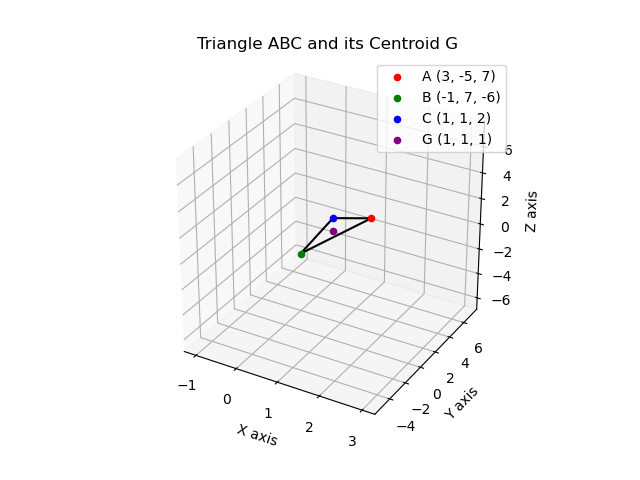
\includegraphics[width=0.7\linewidth]{Figure_1.png}
   \caption{Stem Plot of y\brak{n}}
   \label{stemplot}
\end{figure}





\end{document}
